\documentclass[en,license=none]{../../../eplsummary}

\usepackage{float}

\graphicspath{{img/}}

\hypertitle{Computer networks}{5}{INGI}{1341}
{Gilles Peiffer}
{Olivier Bonaventure}

\part{Principles}
\section{Connecting two hosts}

The first step when building a network,
even a worldwide network such as the Internet,
is to connect two hosts together.
In order for two hosts to exchange information,
they need to be linked by some kind of physical medium.
Various types of media have been used for this purpose:
\begin{itemize}
	\item \emph{Electrical cable}.
	Different types of cables are suitable for transmitting information:
	\begin{itemize}
		\item twisted pairs,
		which are used in the telephone network
		and in enterprise networks;
		\item coaxial cables,
		which are used in cable \textsc{TV} networks,
		but not in enterprise networks anymore.
	\end{itemize}
	Some technologies operate over the classical electrical cable.
	\item \emph{Optical fiber}.
	Optical fibers are used in networks
	when the distance between the devices is larger than one kilometer.
	There are two main types of optical fibers:
	\begin{itemize}
		\item multimode, which uses a \textsc{LED} to send signals
		over distances greater than several tens of kilometers;
		\item monomode, which uses a laser to send signals
		over distances of a few kilometers.
	\end{itemize}
	Both types can use repeaters to regenerate the signal
	and send it over another fiber.
	\item \emph{Wireless}.
	With this technology,
	a radio signal is used to encode the exchanged information.
	Modulation techniques are used
	to send information over a wireless channel.
	Some wireless networks use a laser
	that sends light pulses to a detector
	instead of a radio signal.
	These optical techniques allow to create point-to-point links,
	while radio based techniques can be used
	to build networks containing devices
	spread over a small geographical area.
\end{itemize}

\subsection{The physical layer}

The physical media explained previously can be used to exchange information,
once this information has been converted into a suitable electrical signal.
We will focus on the transmission of bits, i.e. either $0$ or $1$.

\begin{mydef}[Bit rate]
	In computer networks, the bit rate of the physical layer
	is always expressed in bits per second.
	This is in contrast with memory specifications
	which are usually expressed in bytes
	(one byte is equal to eight bits).
\end{mydef}

\subsubsection{Time-sequence diagram}

A physical transmission scheme
(interactions between communicating hosts)
can be described by using a \emph{time-sequence diagram}.
By convention, the sender is represented on the left,
and the receiver is on the right.
The middle of the diagram represents the electrical link.
Time flows from top to bottom.
To represent the transmission of a single bit,
three arrows are needed.
\begin{enumerate}
	\item The sender receives a request to transmit one bit of information.
	A \emph{primitive} is used to represent this request,
	sort of like a procedure call.
	The bit being transmitted is the only parameter.
	In the example in \figuref{timeseqdiag},
	the primitive is named \texttt{DATA.request}.
	\item The dashed arrow indicates the signal's propagation time
	between the two hosts.
	Once the signal is received,
	it's interpreted and converted into a bit.
	\item The bit is delivered as a \texttt{DATA.indication} primitive.
\end{enumerate}

\begin{figure}[H]
	\centering
	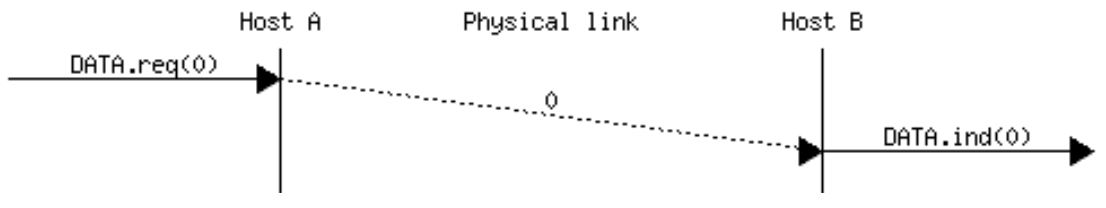
\includegraphics[width=0.5\textwidth]{timeseqdiag.png}
	\caption{A simple time-sequence diagram.}
	\label{fig:timeseqdiag}
\end{figure}

One of the problems of such a transmission scheme
is that electromagnetic interference can switch bits
while they're being transmitted
(i.e. a $0$ bit is sent but a $1$ bit is received).

With the above transmission scheme,
a bit is transmitted by setting the voltage on the electrical cable
to a specific value during some period of time.
One source of errors can be the difference in measured voltage
between the sender and the receiver.
Another reason could be that the two clocks do not operate
at exactly the same frequency.
Small differences in clock frequency imply
that bits can ``disappear'' or ``appear''
during their transmission on an electrical cable
(as in \figuref{lostbitdiag}).

\begin{figure}[H]
	\centering
	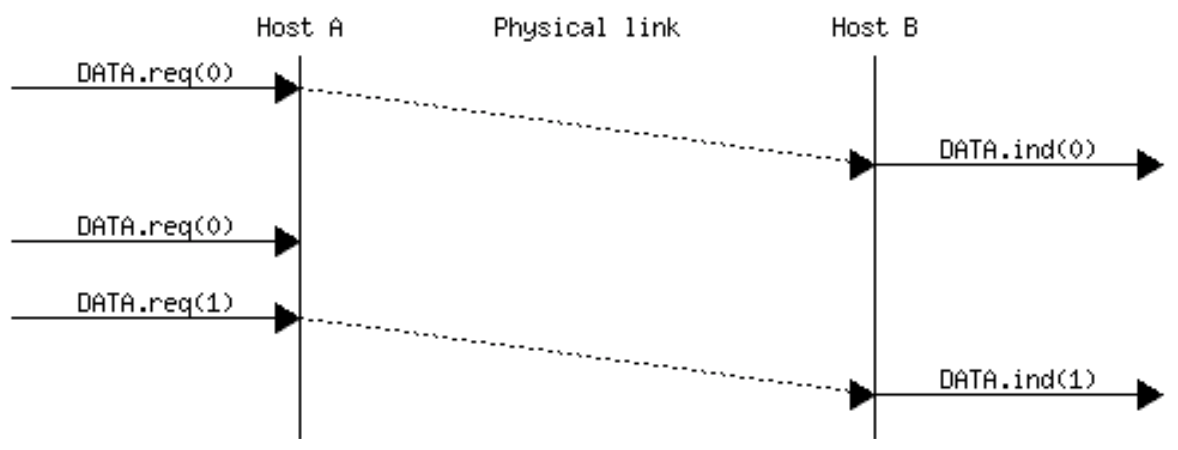
\includegraphics[width=0.5\textwidth]{lostbitdiag.png}
	\caption{Bits can ``disappear'' due to mismatched clock frequencies.}
	\label{fig:lostbitdiag}
\end{figure}

Due to these possible sources of error,
it's important to remember that the physical layer service may
\begin{itemize}
	\item \textbf{change} the value of a bit being transmitted,
	\item \textbf{deliver more (or less)} bits to the receiver
	than the bits sent by the sender.
\end{itemize}

\paragraph{Manchester encoding} Other types of encodings have been defined
to transmit information over an electrical cable.
All physical layers are able to send and receive physical symbols
that represent the values $0$ and $1$.
However, for various reasons that are outside the scope of this chapter,
several physical layers exchange other physical symbols as well.
The Manchester encoding is an encoding scheme
in which time is divided into fixed-length periods.
Each period is divided into two halves
during which different voltage levels (high or low) can be applied.
The four possible combinations make for four possible characters,
as shown in \figuref{manchester_encoding}.

\begin{figure}[H]
	\centering
	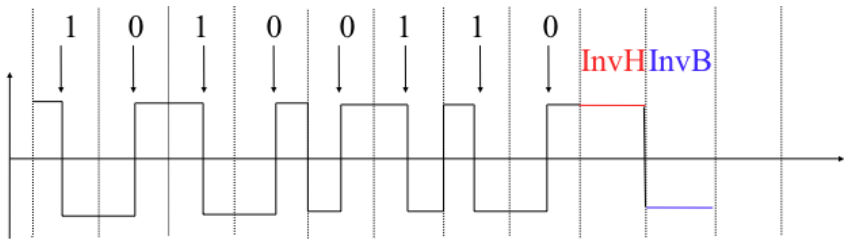
\includegraphics[width=\textwidth]{manchester_encoding.png}
	\caption{Visualisation of the Manchester encoding.
	$0$ and $1$ are regular bits,
	the InvH and InvB symbols can be used as markers
	for the beginning or end of frames.}
	\label{fig:manchester_encoding}
\end{figure}

\subsection{The datalink layer}

The physical layer is the name given
to all the functions related to the physical transmission of information.
It allows two or more entities to exchange bits
if they are connected to the same medium.
Computer networks use different layers,
where each layer provides a service that is built above the underlying layer,
and is close to the needs of the applications.
The datalink layer builds upon the service provided by the physical layer.
\bigbreak
\subsubsection{Framing}
\begin{mydef}[Frame]
	In many networks, the fundamental unit of of information
	exchanged between two hosts is called a \emph{frame}.
	A \emph{frame} is a sequence of bits
	that has a particular syntax or structure.
\end{mydef}
\begin{myrem}[Bit rate and bandwidth]
	Bit rate and bandwidth are often used
	to characterize the transmission capacity of the physical service.
	Bandwidth is defined as ``a range of radio frequencies
	which is occupied by a modulated carrier wave,
	which is assigned to a service,
	or over which a device can operate''.
	By extension, bandwidth is also used
	to represent the capacity of a communication system in bits per second.
\end{myrem}
Since the physical layer is not perfect,
transmitting and receiving frames
is not as simple as just defining a way to encode frames into bits,
or make out frames from bits.
A generic solution exists that works on any physical layer: \emph{stuffing}.
To enable a receiver to easily delineate the frame boundaries,
special bit strings serve as frame boundary markers
and encode the frames so that these special bit strings
do not appear inside the frames.
There are two variants of \emph{stuffing}:
\begin{itemize}
	\item \emph{Bit stuffing}.
	Bit stuffing reserves the $01111110$ bit string
	as the frame boundary marker
	and ensures there will never be six consecutive $1$ symbols
	transmitted by the physical layer inside a frame.
	It works as follows:
	\begin{enumerate}
		\item The sender transmits the marker, i.e. $01111110$.
		\item The sender sends all the bits of the frame
		and inserts an additional bit set to $0$
		after each sequence of five consecutive $1$ bits.
		\item The sender transmits the marker again,
		marking the end of the frame.
		\item The receiver detects the beginning of a frame
		thanks to the marker.
		\item The receiver processes the received bits,
		and if it counts five consecutive bits set to $1$,
		followed by a $0$ bit,
		that last bit is discarded.
		\item Once the receiver detects the marker again,
		it knows the frame has been received entirely.
	\end{enumerate}
	Bit stuffing increases the number of bits
	required to transmit the frame,
	with the worst case being
	a long sequence of bits set to $1$ inside the frame.
	Note that bit stuffing is vulnerable to transmission errors.
	If such an error happens,
	the frame (and possible the next)
	will not correctly be decoded by the receiver,
	but it will be able to resynchronize itself at the next valid marker.
	\item \emph{Character stuffing}.
	Character stuffing techniques
	use control characters in the \textsc{ASCII} table
	as markers to delineate frame boundaries.
	The following markers are often used:
	\textsc{DLE STX} to mark the beginning
	and \textsc{DLE ETX} to mark the end\footnote{\textsc{DLE} ($0010000$ b) for ``Data Link Escape'',
	\textsc{STX} ($0000010$ b) for ``Start of Text''
	and \textsc{ETX} ($0000011$ b) for ``End of Text''.}.
	When transmitting a frame,
	the sender adds a \textsc{DLE} character
	after each transmitted \textsc{DLE} character.
	This ensures that none of the markers
	can appear inside the transmitted frame.
	The receiver detects this
	and removes the second \textsc{DLE}
	when it receives two consecutive ones.
	Just like bit stuffing,
	character stuffing increases the length of the transmitted frames.
	The worst frame for character stuffing
	is a frame containing many \textsc{DLE} characters.
	Again, two frames can potentially be lost
	when a transmission error occurs,
	but the receiver will be able to resynchronize itself
	with the next correctly received markers.
\end{itemize}
While bit stuffing is easily implemented in hardware,
it is difficult to implement in software
given the complexity of performing bit manipulations in software.
Software implementations prefer to use character stuffing instead.

Both of these techniques allow to recover frames from a stream of bits or bytes.
The framing mechanism provides a richer service than the physical layer.
It can also be represented
using the \texttt{DATA.req} and \texttt{DATA.ind} primitives,
as illustrated in \figuref{stuffing_diag}.

\begin{figure}[H]
	\centering
	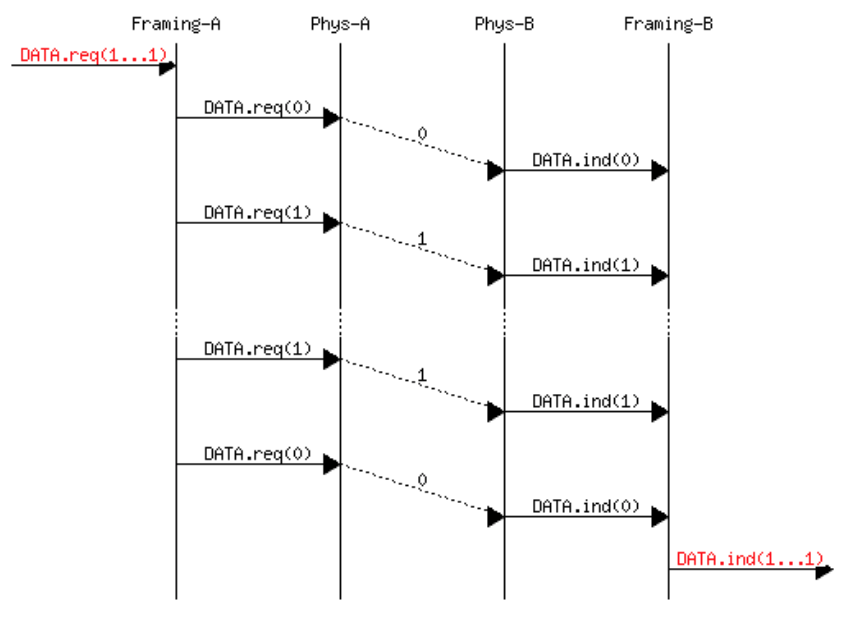
\includegraphics[width=0.4\textwidth]{stuffing_diag.png}
	\caption{Time-sequence diagram of framing,
	assuming hypothetical frames containing four useful bits
	and one bit of framing.}
	\label{fig:stuffing_diag}
\end{figure}

\subsubsection{Recovering from transmission errors}
We distinguish two types of \texttt{DATA.req} and \texttt{DATA.ind} primitives:
\begin{itemize}
	\item the interactions between the user and the datalink layer entity
	are represented using \texttt{DATA.req} and \texttt{DATA.ind};
	\item the interactions between the datalink layer entity
	and the framing sublayer
	are represented by using \texttt{send} and \texttt{recvd}.
\end{itemize}
The datalink layer entity has a buffer
to deal with \textsc{SDU}s\footnote{Service data unit,
a generic term to represent the data that is transported by a protocol.}
that have been received as a \texttt{DATA.request}
but have not been sent.
It also has a buffer that deals with received frames
that haven't been processed yet.
If one of these buffers overflows,
arriving frames will be discarded,
even if they are correct.
Hence, a reliable protocol must include a feedback mechanism
that allows the receiver to inform the sender that it has processed a frame
and that another one can be sent,
regardless of transmission errors.
We need two types of frames:
\begin{itemize}
	\item \emph{data frames} carrying an \textsc{SDU};
	\item \emph{control frames} carrying an acknowledgment
	indicating the previous frames were processed correctly.
\end{itemize}
These two types can be distinguished by dividing the frame in two parts:
\begin{itemize}
	\item the \emph{header} that contains a bit
	set to $0$ in data frames and $1$ in control frames.
	\item the \emph{payload} that contains the \textsc{SDU}
	supplied by the application.
\end{itemize}
The datalink entity can then be modelled
as an \textsc{FSM}\footnote{Finite state machine.},
containing two states for the receiver and the sender (\figuref{fsm}).

\begin{figure}[H]
	\centering
	\begin{subfigure}[t]{0.45\linewidth}
		\centering
		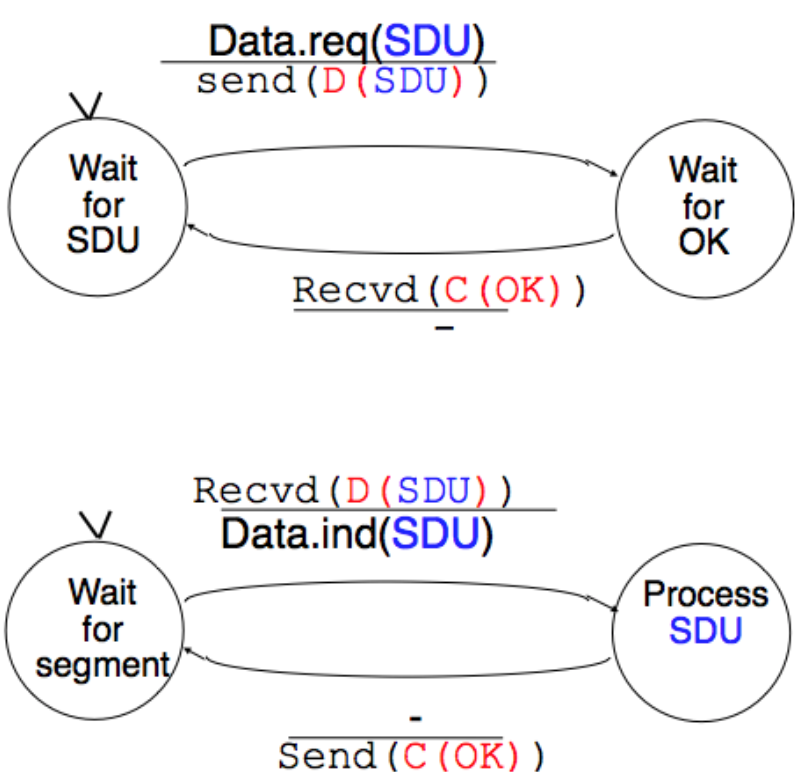
\includegraphics[width=0.6\textwidth]{fsm.png}
		\caption{\textsc{FSM} of the simplest reliable protocol,
		with the sender above and the receiver below.
		The sender has to wait for an acknowledgment
		before being able to transmit the next \textsc{SDU}.}
		\label{fig:fsm}
	\end{subfigure}
	\hfill
	\begin{subfigure}[t]{0.45\linewidth}
		\centering
		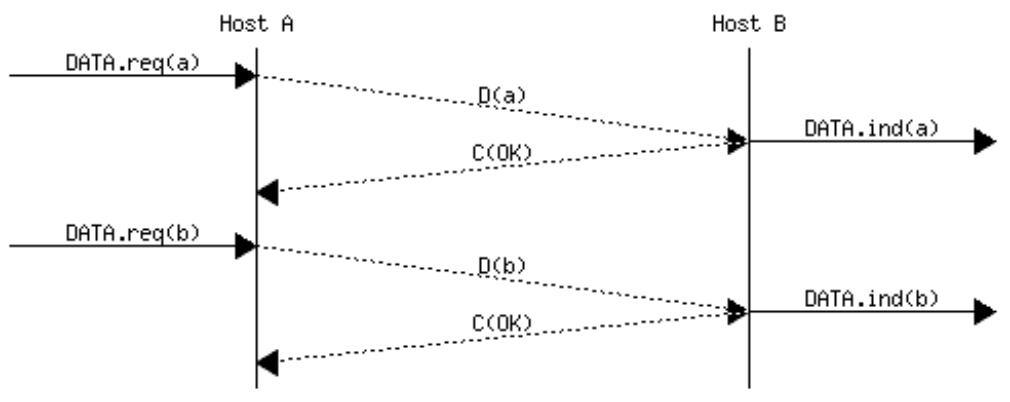
\includegraphics[width=\textwidth]{simp_rel_prot.png}
		\caption{Exchange of a few frames between two hosts.}
		\label{fig:simp_rel_prot}
	\end{subfigure}
\end{figure}

\subsubsection{Reliable data transfer on top of an imperfect link}
In the datalink layer,
we mainly have to deal with two types of transmission errors:
\begin{itemize}
	\item corrupted frames;
	\item lost or unexpected frames;
\end{itemize}
Data transmission on a physical link
can be affected by the following transmission errors:
\begin{itemize}
	\item random isolated errors
	where the value of a single bit has been modified;
	\item random burst errors
	where the values of $n$ consecutive bits have been changed;
	\item random bit creations and removals.
\end{itemize}
In order to avoid this,
we have to add \emph{redundancy} to the frames that are sent.
Information theory allows us to add redundant information
as an \emph{error detection code}.
Simply put,
the frame is sent with an error detection code,
computed by the sender, added to it.
Once the frame is received,
the receiver recomputes the error detection code
and verifies whether it matches the received one.
To understand error detection codes,
consider two devices that exchange bit strings containing $N$ bits.
To allow the receiver to detect a transmission error,
an error detection code calculates $r$ redundant bits
for each string of $N$ bits,
thus transforming the strings into strings of $N+r$ bits each.
The simplest error detection code is the parity bit.
Two types exist: even and odd parity.
With the even (resp. odd) parity scheme,
the redundant bit is chosen so that an even (resp. odd) number of bits
are set to $1$ in the transmitted string.
The receiver can easily recompute the parity of each received bit string
and discard the strings with an invalid parity.
This means that if multiple bits have been affected,
the receiver might not be able to detect the transmission error.
Another example of a (more powerful) error detection code
is a \textsc{CRC}\footnote{Cyclic redundancy check.},
which are widely used in datalink layer protocols.
\begin{myprop}[CRC]
	An $N$-bit \textsc{CRC} can detect
	\begin{itemize}
		\item all transmission errors affecting a burst
		of less than $N$ bits in the transmitted frame and
		\item all transmission errors that affect an odd number of bits.
	\end{itemize}
\end{myprop}

It is also possible to design a code
that allows the receiver to correct transmission errors,
the simplest example of which being
the \textsc{TMR}\footnote{Triple modular redundancy.},
where every bit is sent three consecutive times,
so as to allow the receiver to detect errors
and correct them by looking at the majority of bits in case an error occurs.
Other more powerful codes like the Hamming Code,
which is a clever combination of parity bits, exist.
However, these error correction schemes aren't really used in practice.

A frame is usually divided into two parts:
\begin{itemize}
	\item A \emph{header} that contains
	the fields used by the reliable protocol to ensure reliable delivery.
	The header contains a checksum or \textsc{CRC}
	that is used to detect transmission errors.
	Some headers also indicate a \emph{length field}
	with the length of the frame or the payload.
	\item A \emph{payload} that contains the user data.
\end{itemize}
The checksum is a simple error detection scheme:
both the sender and the receiver compute the arithmetic sum
of all the bytes of the frame.
Frames with an invalid checksum are discarded by the receiver.
\textsc{CRC}s have better error detection capabilities,
but require more processing power when implemented in software.
\begin{myrem}[Checksums and \textsc{CRC}s]
	Both checksums and \textsc{CRC}s are used in practice.
	The \textsc{TCP/IP} and \textsc{OSI} communities chose checksums
	(resp. the Internet checksum and the Fletcher checksum),
	while many datalink layer protocols and file formats such as
	\texttt{zip} or \texttt{png} use \textsc{CRC}s.
	It always comes down to a trade-off between error detection capabilities
	and processing power.
\end{myrem}

Since the receiver send an acknowledgment after each received data frame,
a retransmission timer is used.
The value of this retransmission timer needs to be larger
than the \textsc{RTT}\footnote{Round-trip time,
i.e. the delay between the transmission of the first bit of a data frame
to the reception of the last bit of the corresponding acknowledgment.}.
A retransmission timer is started when the sender sends a frame,
and when it expires,
the sender assumes the data segment was lost
and retransmits it (\figuref{retrans_timer}).
\begin{figure}[H]
	\centering
	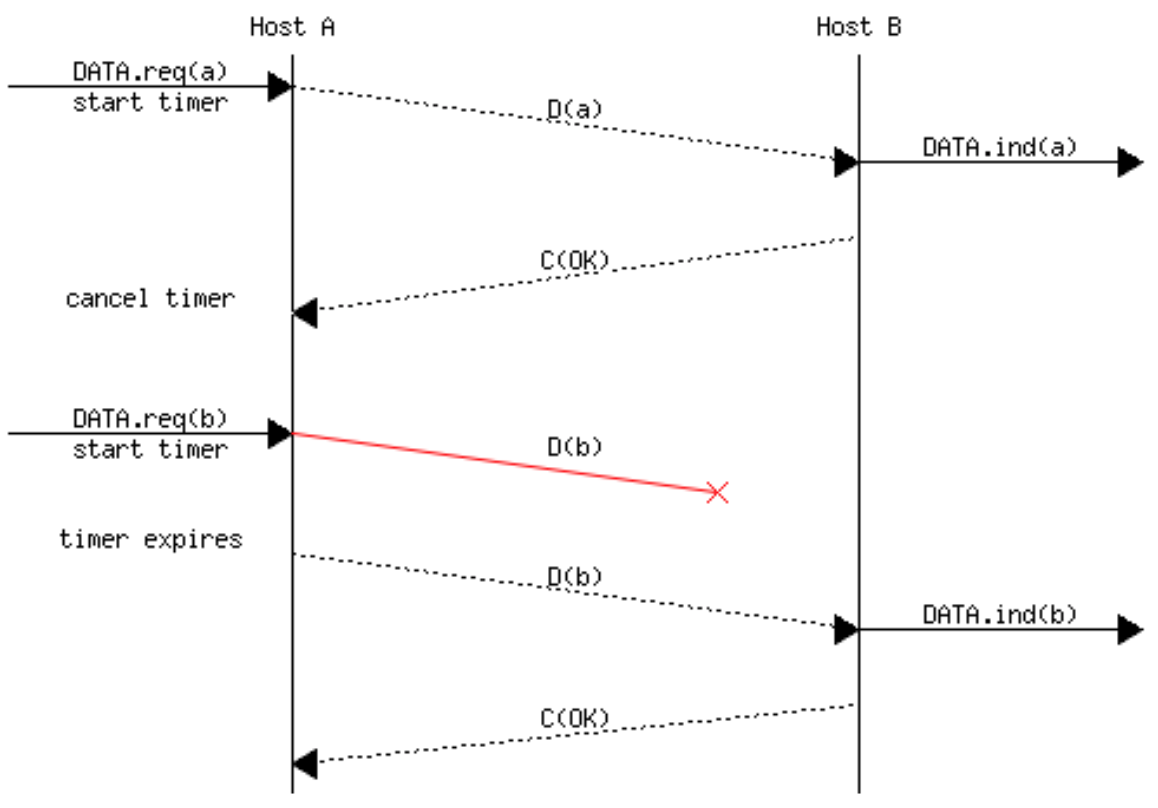
\includegraphics[width=0.4\textwidth]{retrans_timer.png}
	\caption{An example of retransmission timer expiry.}
	\label{fig:retrans_timer}
\end{figure}

However, an issue that can (and does) arise,
is the case when the acknowledgment is lost.
If this happens,
the sender will retransmit the data segment,
except that the receiver will interpret this retransmission as a new segment,
whose payload must be delivered to the user.
To solve this problem,
datalink protocols associate a seqnum\footnote{Sequence number.}
to each data frame.
This seqnum is one of the fields in the header of data frames.
We use the notation \texttt{D(x,\dots)}
to indicate a data frame whose seqnum field is set to value \texttt{x}.
The sequence number is encoded as a bit string of fixed length.
A simple reliable protocol
is \emph{Alternating bit protocol} (\textsc{ABP}).

\textsc{ABP} uses a single bit to encode the seqnum.
The sender and receiver
only require a four-state \textsc{FSM} (\figuref{abp_fsm}).

\begin{figure}[H]
	\centering
	\begin{subfigure}[t]{0.45\linewidth}
		\centering
		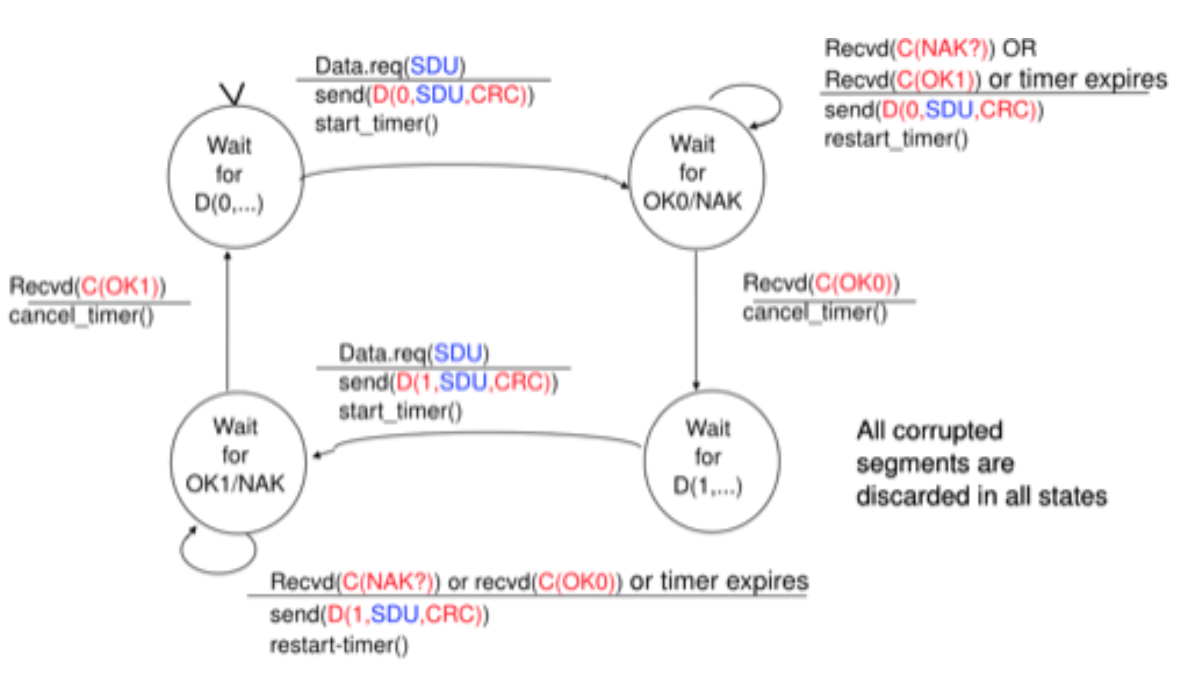
\includegraphics[width=\textwidth]{abp_sender_fsm.png}
		\caption{\textsc{ABP} sender \textsc{FSM}.
		The initial state of the sender
		is \texttt{Wait for D(0,\dots)}.
		In this state,
		the sender waits for a \texttt{DATA.request}.
		The first data frame uses seqnum $0$.
		Once this is sent,
		the sender waits for an \texttt{OK0} acknowledgment.
		A frame is transmitted when the retransmission timer expires
		or when an acknowledgment with an incorrect seqnum
		has been received.}
		\label{fig:abp_sender_fsm}
	\end{subfigure}
	\hfill
	\begin{subfigure}[t]{0.45\linewidth}
		\centering
		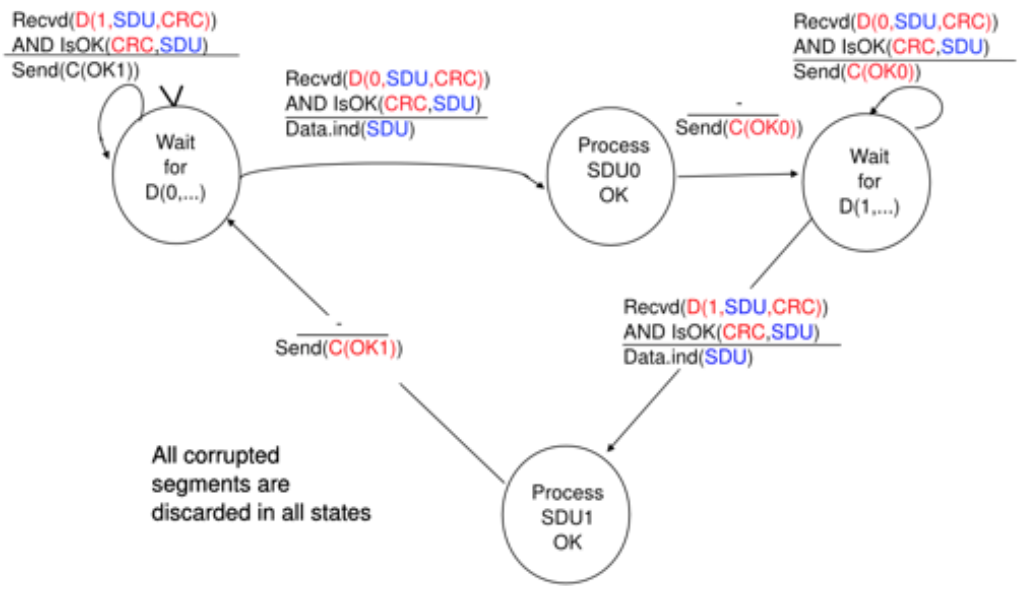
\includegraphics[width=\textwidth]{abp_receiver_fsm.png}
		\caption{\textsc{ABP} receiver \textsc{FSM}.
		The receiver first waits for \texttt{D(0,\dots)}.
		If the frame contains a correct \textsc{CRC},
		it passes the \textsc{SDU} to its user and sends \texttt{OK0}.
		If the \textsc{CRC} is invalid,
		the frame is discarded.
		The receiver then waits for \texttt{D(1,\dots)}.
		In this state,
		it may receive a duplicate \texttt{D(0,\dots)}
		or a data frame with an invalid \textsc{CRC}.
		In both cases, it returns an \texttt{OK0} frame
		to allow the sender to recover
		from the possible loss of the previous \texttt{OK0} frame.}
		\label{fig:abp_receiver_fsm}
	\end{subfigure}
	\caption{\textsc{FSM}s for the \textsc{ABP}.}
	\label{fig:abp_fsm}
\end{figure}

\textsc{ABP} can recover
from transmission errors and frame losses (shown in \figuref{abp_errors}).
However, it has an important drawback:
it has low maximum throughput.

\begin{figure}[H]
	\centering
	\begin{subfigure}[t]{0.31\linewidth}
		\centering
		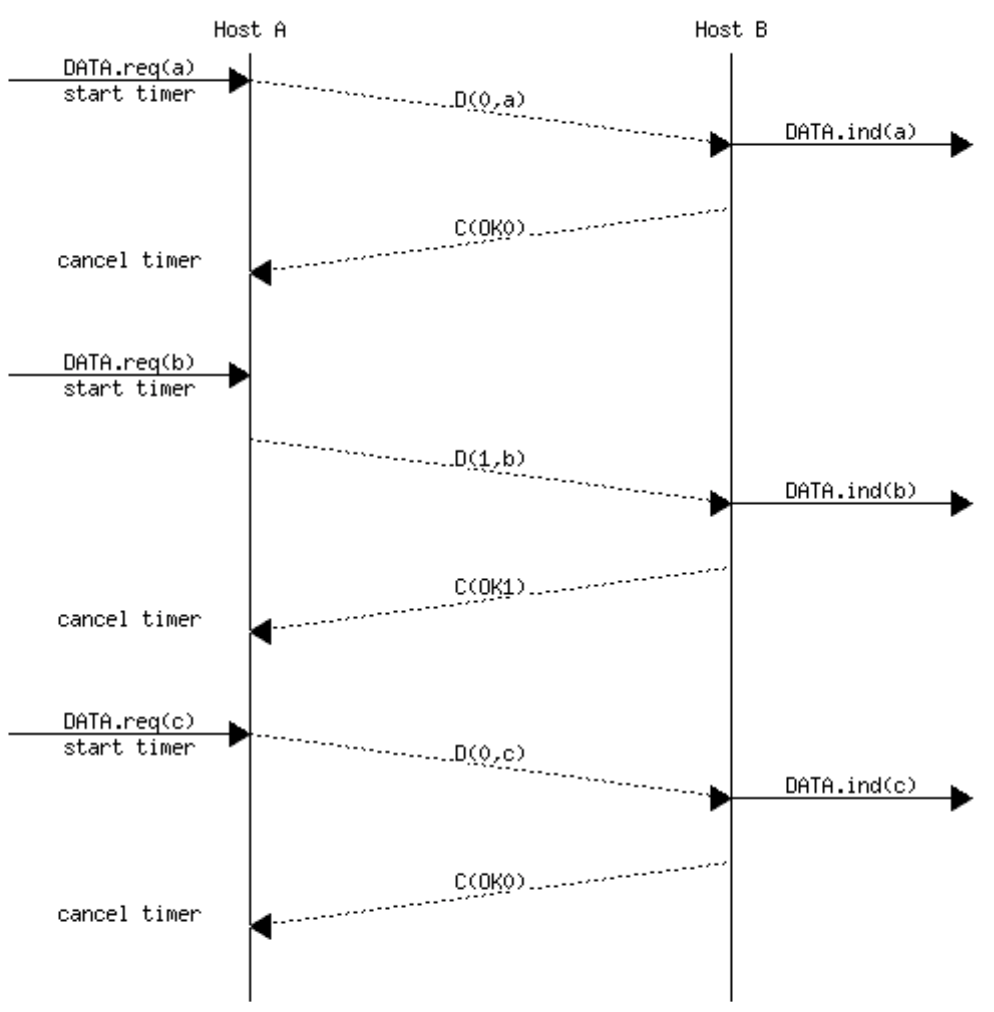
\includegraphics[width=\textwidth]{abp_success.png}
		\caption{A successful transmission with \textsc{ABP}.}
		\label{fig:abp_success}
	\end{subfigure}
	\hfill
	\begin{subfigure}[t]{0.31\linewidth}
		\centering
		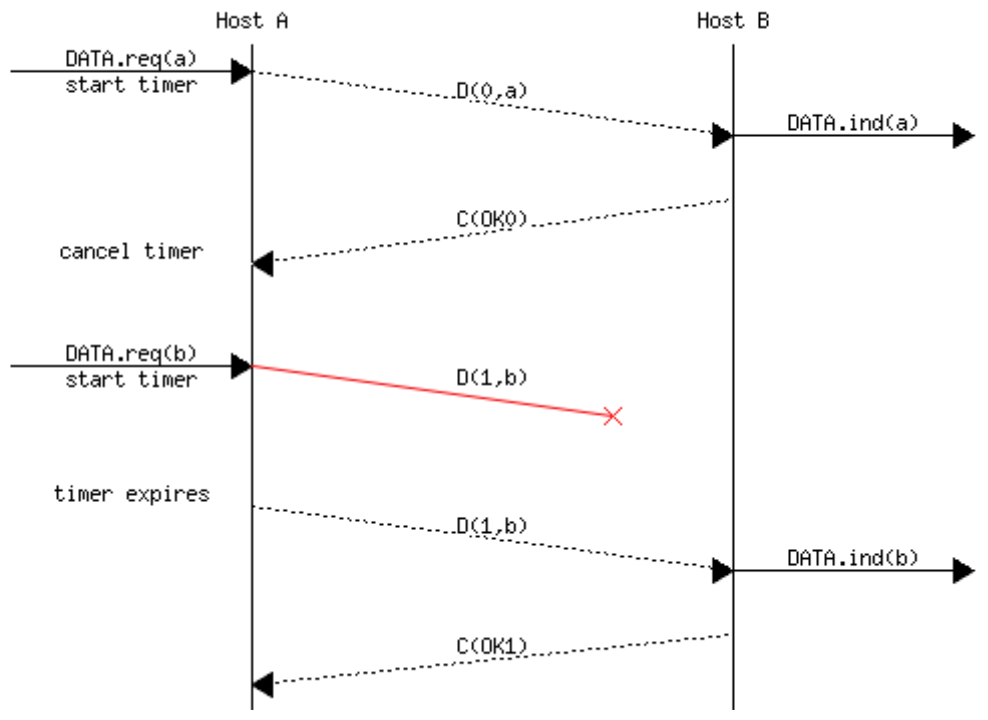
\includegraphics[width=\textwidth]{abp_error_trans.png}
		\caption{\textsc{ABP} can recover from the loss of data frames.}
		\label{fig:abp_error_trans}
	\end{subfigure}
	\hfill
	\begin{subfigure}[t]{0.31\linewidth}
		\centering
		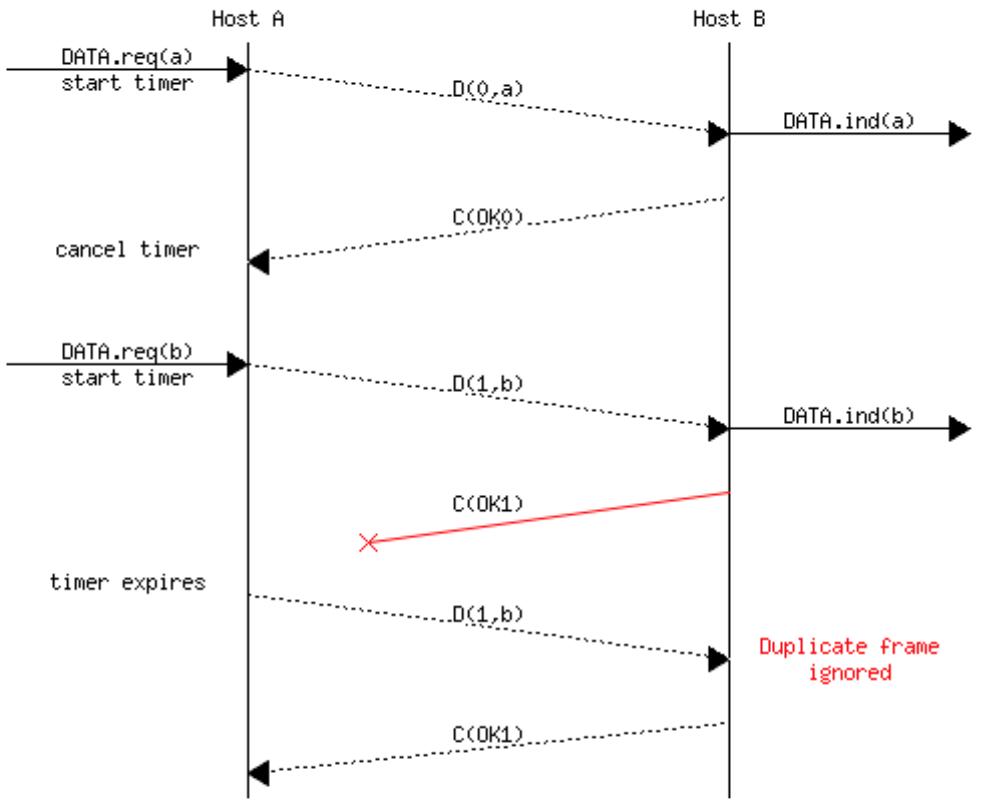
\includegraphics[width=\textwidth]{abp_error_ack.png}
		\caption{\textsc{ABP} can recover
		from the loss of control frames.}
		\label{fig:abp_error_ack}
	\end{subfigure}
	\caption{\textsc{ABP} can recover
	from the losses of data or control frames.}
	\label{fig:abp_errors}
\end{figure}
\subsubsection{Go Back $N$}
To deal with the performance limitations of \textsc{ABP},
reliable protocols rely on \emph{pipelining}.
This means a sender can send multiple consecutive frames
without having to wait for an acknowledgment after each frame.
Each frame contains a seqnum encoded in an $n$-bit field.
Pipelining can possibly overload the receiver,
which is why reliable protocols only allow
$W$ unacknowledged frames to be transmitted
before being forced to wait for an acknowledgment.
This is implemented by using a \emph{sliding window},
like the ones shown in \figuref{sliding_window}.

\begin{figure}[H]
	\centering
	\begin{subfigure}[t]{0.45\linewidth}
		\centering
		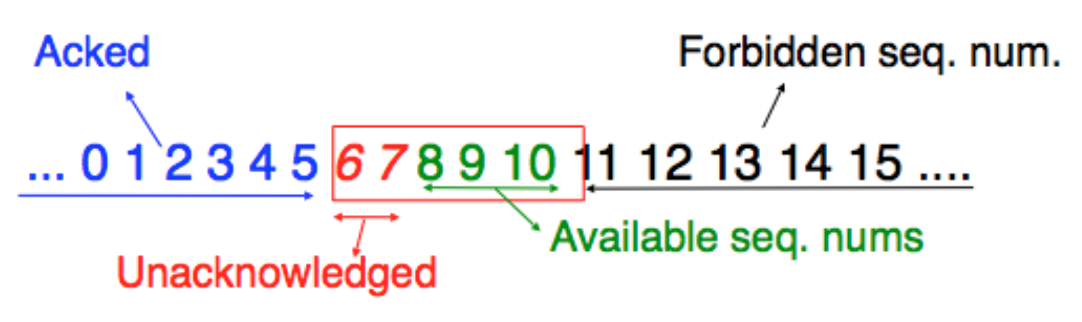
\includegraphics[width=\textwidth]{sliding_window1.png}
		\caption{An example sliding window containing $5$ segments.}
		\label{fig:sliding_window1}
	\end{subfigure}
	\hfill
	\begin{subfigure}[t]{0.45\linewidth}
		\centering
		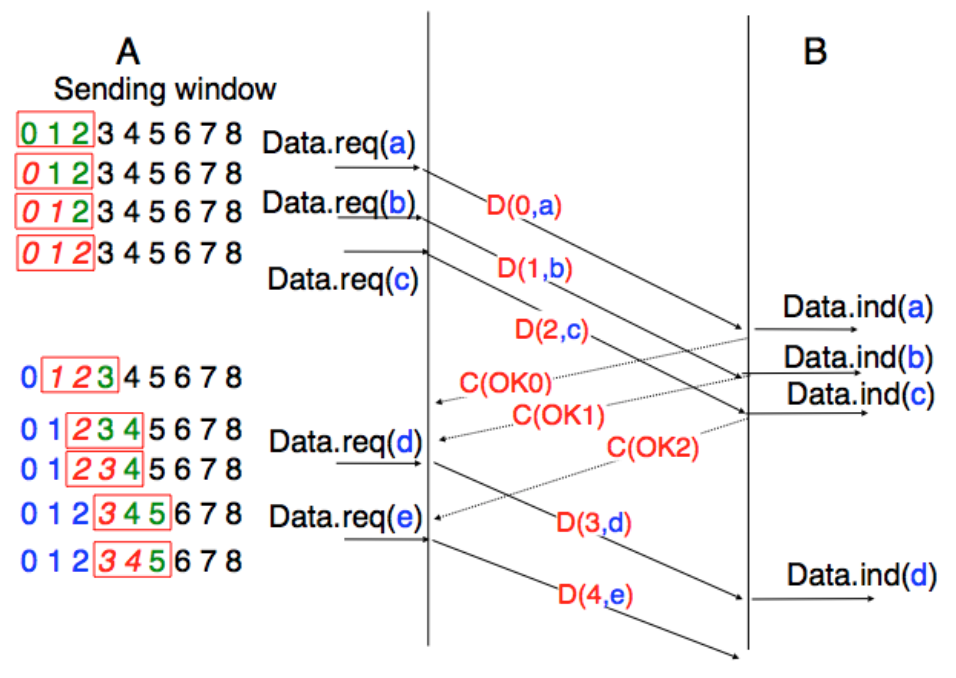
\includegraphics[width=\textwidth]{sliding_window2.png}
		\caption{An example of a sliding window of size $3$
		being used by the sender.}
		\label{fig:sliding_window2}
	\end{subfigure}
	\caption{The sliding window.}
	\label{fig:sliding_window}
\end{figure}

Note that since the headers use an $n$-bit field to encode the seqnum,
only the numbers in the interval $0$--$2^n - 1$ can be used.
This means the sliding window needs to be able to wrap.

To recover from losses,
a sliding window protocol must define
\begin{itemize}
	\item a \emph{heuristic} to detect frame losses and
	\item a \emph{retransmission strategy} to retransmit the lost frames.
\end{itemize}
The simplest such strategy is called Go Back $N$.
It works as follows:
when a receiver receives a frame,
it returns an acknowledgment containing the seqnum of
the last in-sequence frame it received.
This acknowledgment is said to be \emph{cumulative}.
This means that if the frame with seqnum $x$ is acknowledged,
then the sender knows that all previous frames were also received succesfully,
even if their acknowledgments were lost in transmission.
A sender stores a buffer of the size of the sliding window.
The frames are sent with increasing seqnums
($\mod \texttt{maxseq}$).\footnote{\texttt{maxseq} is the maximum number of different sequence numbers ($2^n$).}
Once the sending buffer is full,
it must wait for an acknowledgment.
When the sender receives an acknowledgment,
it removes all the acknowledged frames from the sending buffer,
and uses a retransmission timer to detect frame losses.
This timer is started when the first frame is sent,
and after receicing an acknowledgment,
it only restarts the timer if
there are still unacknowledged frames in the sending buffer.
When the timer expires,
all frames in the buffer are retransmitted
(and the timer is restarted again, etc.).
These possible states are summarized in \figuref{gbn_fsms}.

\begin{figure}[H]
	\centering
	\begin{subfigure}[t]{0.45\linewidth}
		\centering
		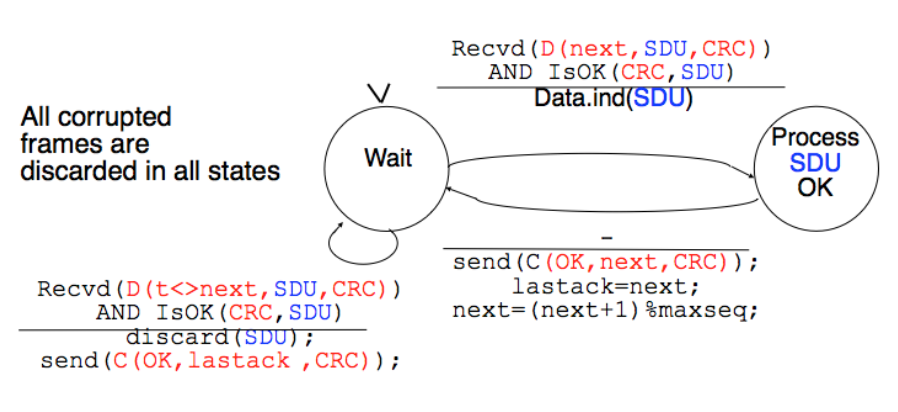
\includegraphics[width=\textwidth]{gbn_receiver_fsm.png}
		\caption{The finite state machine for a Go Back $N$ receiver.
		This receiver uses two variables:
		\texttt{lastack} and \texttt{next}.
		\texttt{next} is the next expected sequence number
		and \texttt{lastack} the sequence number
		of the last data frame that has been acknowledged.
		The receiver only accepts the frames
		that are received in sequence.}
		\label{fig:gbn_receiver_fsm}
	\end{subfigure}
	\hfill
	\begin{subfigure}[t]{0.45\linewidth}
		\centering
		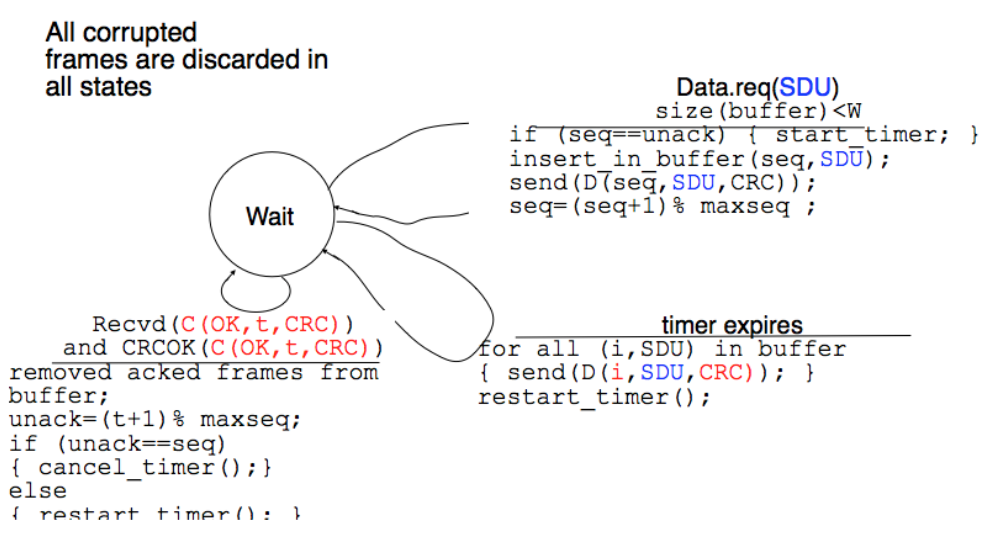
\includegraphics[width=\textwidth]{gbn_sender_fsm.png}
		\caption{The finite state machine for a Go Back $N$ sender.}
		\label{fig:gbn_sender_fsm}
	\end{subfigure}
	\caption{Finite state machines for the Go Back $N$ recovery protocol.}
	\label{fig:gbn_fsms}
\end{figure}

The operation of this protocol is illustrated in \figuref{gbn_ex}.
\begin{figure}[H]
	\centering
	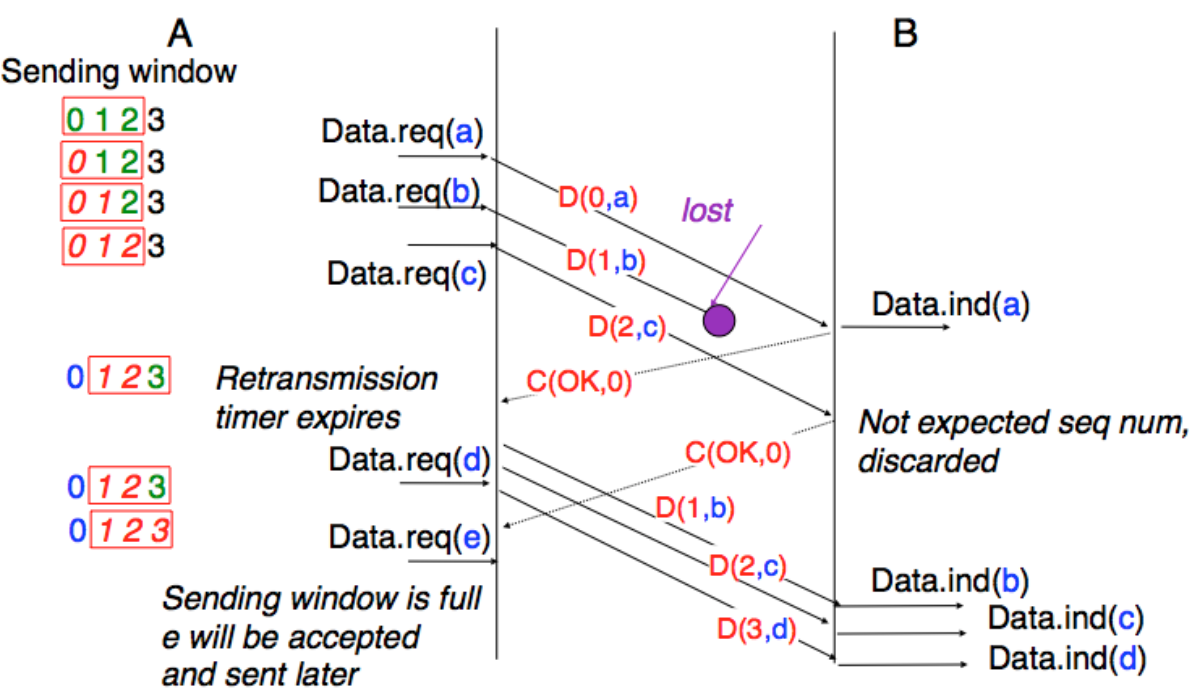
\includegraphics[width=0.6\textwidth]{gbn_ex.png}
	\caption{An example of Go Back $N$ at work.}
	\label{fig:gbn_ex}
\end{figure}

While it is easy to implement,
Go Bac $N$ also has some drawbacks:
when many frames are lost,
performance drops because out-of-sequence frames
are not accepted by the receiver and
the sender retransmits \emph{all} frames once it detects a loss.
\subsubsection{Selective repeat}
For these reasons,
selective repeat is a smarter strategy.
It has a sliding window of $W$ frames,
just like Go Back $N$,
but it also stores received out-of-frequence frames.
The selective repeat receiver discards all frames with an invalid \textsc{CRC}.
\texttt{lastack} is the last in-sequence frame received,
and it is always included in the acknowledgments that the receiver sends.
Some protocols also allow the selective repeat receiver
to acknowledge the out-of sequence frames that it has received.
This can be done by placing the list of the correctly received,
but out-of-sequence frames together with the \texttt{lastack} value.
When the receiver receives a data frame,
it first verifies whether the frame is inside its receiving window.
If yes, the frame is placed in the receive buffer.
If not, the frame is discarded and an acknowledgment with \texttt{lastack}
is sent to the sender.
The receiver then removes all consecutive frames
starting at \texttt{lastack} (if any) from the receive buffer.
The payloads of these frames are delivered to the user,
\texttt{lastack} and the receiving window are updated,
and an acknowledgment acknowledging the last frame received in sequence is sent.
\bigbreak
The selective repeat sender maintains a sending buffer
that can store up to $W$ unacknowledged frames.
These frames are sent as long as the sending buffer is not full.
Several implementations of a selective repeat sender are possible.
A simple implementation associates one retransmission timer to each frame.
The timer is started when the frame is sent
and cancelled upon reception of an acknowledgement that covers this frame.
When a retransmission timer expires,
the corresponding frame is retransmitted
and this retransmission timer is restarted.
When an acknowledgement is received,
all the frames that are covered by this acknowledgement
are removed from the sending buffer and the sliding window is updated.

\begin{figure}[H]
	\centering
	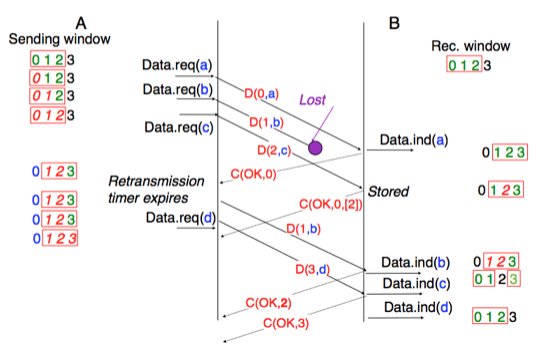
\includegraphics[width=0.6\textwidth]{selective_repeat_ex.png}
	\caption{An example of selective repeat at work.
	The figure illustrates the operation of selective repeat
	when frames are lost.
	In this figure, \texttt{C(OK,x)} is used to indicate that all frames,
	up to and including sequence number $x$ have been received correctly.
	This figure also shows selective acknowledgment,
	which the receiver telling the sender
	about correctly received,
	but out-of-sequence frames.
	The sender knows it should stop the retransmission timers
	for those frames,
	while still keeping them in the sending buffer
	until the reception of a cumulative acknowledgment.}
	\label{fig:selective_repeat_ex}
\end{figure}

\begin{myrem}[Maximum window size with Go Back $N$ and selective repeat]
	Theoretically, the maximum window size for a reliable protocol
	using $n$ bits to encode its seqnums is $2^n$.
	However, consider Go Back $N$ and that all acknowledgments are lost,
	despite the frames being received in-sequence.
	The sender will have to send all the frames again,
	and the user will receive them a second time,
	thinking they're the next batch of frames.
	This can be fixed by using $2^n-1$ instead.
	Something similar happens with selective repeat.
	To avoid this problem and have reliable delivery,
	selective repeat senders should use window of size at most $2^{n-1}$,
	so that the same frame doesn't get accepted multiple times.
\end{myrem}

Reliable protocols often need to send data in both directions.
\emph{Piggybacking} is used to avoid overhead caused by acknowledgments
by allowing the acknowledgments to be sent together with other information.
This only works when data flows in both directions.
If no data is to be sent,
the receiver will simply send a pure acknowledgment (\figuref{piggybacking}).
\begin{figure}[H]
	\centering
	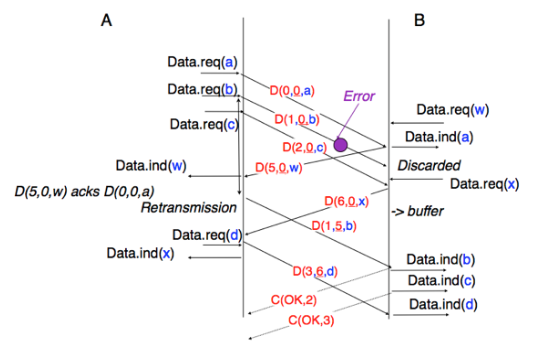
\includegraphics[width=0.6\textwidth]{piggybacking.png}
	\caption{An example of piggybacking being used.
	The bottom of the figure shows
	the receiver sending a pure acknowlegment
	when no data is to be sent in the opposite direction.}
	\label{fig:piggybacking}
\end{figure}

\section{Building a network}
When hosts aren't connected to each other by a direct physical layer link,
we need to add another layer on top of the datalink layer:
the network layer.

Its main objective is to allow end systems,
connected to different networks,
to exchange information through intermediate systems called routers.
Information is sent in packets in the network layer.

Datalink layers can be either reliable
(if the physical layer is prone to suffer from transmission errors)
or unreliable (if transmission errors are rare).
We assume here that the datalink layer service
provides an \emph{almost reliable} service.

There are two main types of datalink layers:
\begin{itemize}
	\item \emph{Point-to-point} datalink layers are used
	when there are only two communicating systems
	that are directly connected through the physical layer.
	Depending on how high the bit error ratio in the physical layer is,
	the datalink layer will be either reliable or unreliable.
	Point-to-point datalink layers can
	either connect two end systems or two routers.
	\item \textsc{LAN}s\footnote{Local area network} use
	a second type of datalink layer.
	A \textsc{LAN} is a set of communicating devices
	such that any two devices
	can directly exchange frames through the datalink layer.
\end{itemize}

Each datalink layer is characterized by a maximum frame size.
The heterogeneity in the maximum frame sizes can cause problems
when we need to exchange data between hosts
attached to different types of datalink layers.

An example network is represented in \figuref{typ_network}.
\begin{figure}[H]
	\centering
	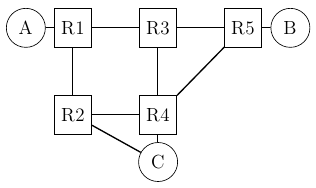
\includegraphics[width=0.4\textwidth]{typ_network.png}
	\caption{A typical network consisting of
	three end systems (or hosts, represented with circles)
	and five routers (represented with boxes).}
	\label{fig:typ_network}
\end{figure}

\begin{mydef}[End system]
	\emph{End systems}, or \emph{hosts},
	are devices which are able to send and receive data for their own usage.
	They are usually attached to the network via a single link.
	A host is \emph{multihomed} if it is equipped
	with several physical interfaces.
\end{mydef}
\begin{mydef}[Router]
	\emph{Routers}, in contrast with hosts,
	usually forward data towards its final destination.
	A router has multiple neighboring routers or hosts.
\end{mydef}

Let's analyze the operations that need to be performed to allow host $A$
in the bove network to send one byte to host $B$.
Host $A$ can easily send a frame to router $R1$ over the datalink layer.
The network layer serves to let $R1$ know
that the data is for host $B$ and not for the router itself.

The network layer sends packets from host to host,
with intermediate routers in between.
Packets contain the information to be transmitted
as well as control information.
Each node in the network has an address
(usually a sequence of bits of fixed length).

The packet that host $A$ sends to host $B$
either contains the addresses of the source and the destination nodes,
or information that indicates the path that needs to be followed
to reach the destination.

There are two possible organisations for the network layer:
\begin{itemize}
	\item the \emph{datagram organisation} and
	\item \emph{virtual circuits}.
\end{itemize}

\subsection{The datagram organisation}

\end{document}
